\documentclass{standalone}
\usepackage{tikz}
\usetikzlibrary{patterns, positioning}


\begin{document}
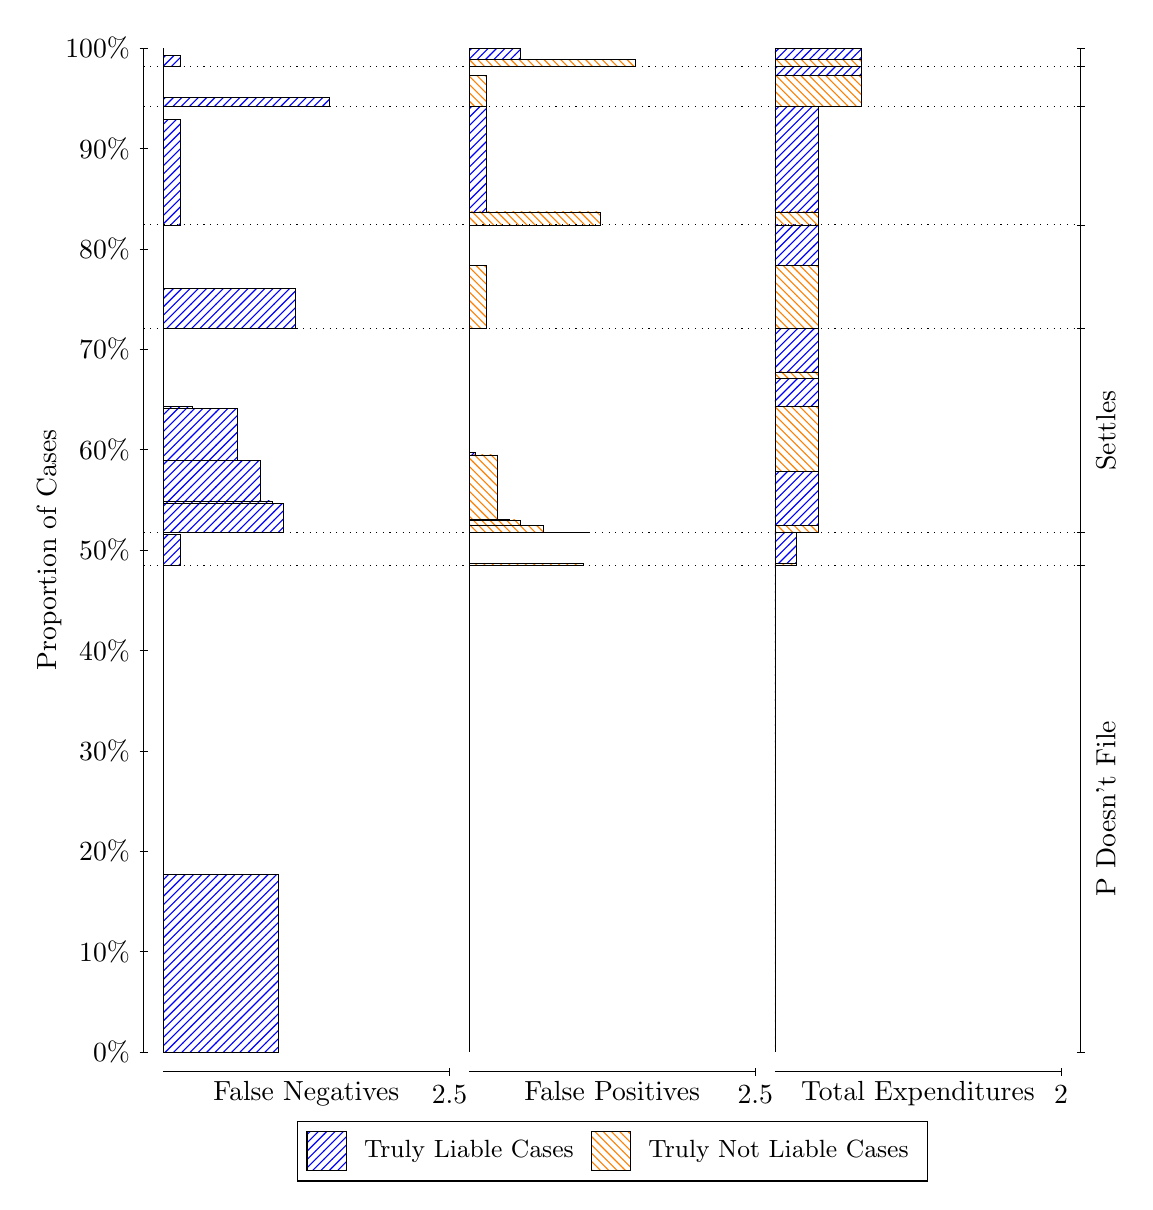
\begin{tikzpicture}
\draw[black, very thin] (1.5,1.75) -- (1.5,14.5);
\node[rotate=90, text=black, anchor=center] at (0.3, 8.125) {Proportion of Cases};
\draw[black, very thin] (1.45,1.75) -- (1.55,1.75);
\node[text=black, anchor=east] at (1.45, 1.75) {0\%};
\draw[black, very thin] (1.45,3.025) -- (1.55,3.025);
\node[text=black, anchor=east] at (1.45, 3.025) {10\%};
\draw[black, very thin] (1.45,4.3) -- (1.55,4.3);
\node[text=black, anchor=east] at (1.45, 4.3) {20\%};
\draw[black, very thin] (1.45,5.575) -- (1.55,5.575);
\node[text=black, anchor=east] at (1.45, 5.575) {30\%};
\draw[black, very thin] (1.45,6.85) -- (1.55,6.85);
\node[text=black, anchor=east] at (1.45, 6.85) {40\%};
\draw[black, very thin] (1.45,8.125) -- (1.55,8.125);
\node[text=black, anchor=east] at (1.45, 8.125) {50\%};
\draw[black, very thin] (1.45,9.4) -- (1.55,9.4);
\node[text=black, anchor=east] at (1.45, 9.4) {60\%};
\draw[black, very thin] (1.45,10.675) -- (1.55,10.675);
\node[text=black, anchor=east] at (1.45, 10.675) {70\%};
\draw[black, very thin] (1.45,11.95) -- (1.55,11.95);
\node[text=black, anchor=east] at (1.45, 11.95) {80\%};
\draw[black, very thin] (1.45,13.225) -- (1.55,13.225);
\node[text=black, anchor=east] at (1.45, 13.225) {90\%};
\draw[black, very thin] (1.45,14.5) -- (1.55,14.5);
\node[text=black, anchor=east] at (1.45, 14.5) {100\%};

\draw[black, very thin] (13.4,1.75) -- (13.4,14.5);
\draw[black, very thin] (13.35,1.75) -- (13.45,1.75);
\node[anchor=west] at (13.35, 1.75) {};
\draw[black, very thin] (13.35,7.9307) -- (13.45,7.9307);
\node[anchor=west] at (13.35, 7.9307) {};
\draw[black, very thin] (13.35,8.3489) -- (13.45,8.3489);
\node[anchor=west] at (13.35, 8.3489) {};
\draw[black, very thin] (13.35,10.935) -- (13.45,10.935);
\node[anchor=west] at (13.35, 10.935) {};
\draw[black, very thin] (13.35,12.255) -- (13.45,12.255);
\node[anchor=west] at (13.35, 12.255) {};
\draw[black, very thin] (13.35,13.762) -- (13.45,13.762);
\node[anchor=west] at (13.35, 13.762) {};
\draw[black, very thin] (13.35,14.262) -- (13.45,14.262);
\node[anchor=west] at (13.35, 14.262) {};
\draw[black, very thin] (13.35,14.5) -- (13.45,14.5);
\node[anchor=west] at (13.35, 14.5) {};

\draw[black, very thin, pattern color=blue, pattern=north east lines] (1.75,1.75) rectangle (3.2033,4.0074);
\draw[black, very thin, pattern color=orange, pattern=north west lines] (1.75,4.0074) rectangle (1.75,7.9307);
\draw[black, very thin, pattern color=blue, pattern=north east lines] (1.75,7.9307) rectangle (1.968,8.3257);
\draw[black, very thin, pattern color=orange, pattern=north west lines] (1.75,8.3257) rectangle (1.75,8.3489);
\draw[black, very thin, pattern color=blue, pattern=north east lines] (1.75,8.3489) rectangle (3.276,8.7122);
\draw[black, very thin, pattern color=blue, pattern=north east lines] (1.75,8.7122) rectangle (3.1307,8.748);
\draw[black, very thin, pattern color=blue, pattern=north east lines] (1.75,8.748) rectangle (2.9853,9.2601);
\draw[black, very thin, pattern color=blue, pattern=north east lines] (1.75,9.2601) rectangle (2.6947,9.9237);
\draw[black, very thin, pattern color=blue, pattern=north east lines] (1.75,9.9237) rectangle (2.5493,9.9243);
\draw[black, very thin, pattern color=blue, pattern=north east lines] (1.75,9.9243) rectangle (2.1133,9.9518);
\draw[black, very thin, pattern color=orange, pattern=north west lines] (1.75,9.9518) rectangle (1.75,10.935);
\draw[black, very thin, pattern color=blue, pattern=north east lines] (1.75,10.935) rectangle (3.4213,11.451);
\draw[black, very thin, pattern color=orange, pattern=north west lines] (1.75,11.451) rectangle (1.75,12.255);
\draw[black, very thin, pattern color=blue, pattern=north east lines] (1.75,12.255) rectangle (1.968,13.597);
\draw[black, very thin, pattern color=orange, pattern=north west lines] (1.75,13.597) rectangle (1.75,13.762);
\draw[black, very thin, pattern color=blue, pattern=north east lines] (1.75,13.762) rectangle (3.8573,13.877);
\draw[black, very thin, pattern color=orange, pattern=north west lines] (1.75,13.877) rectangle (1.75,14.262);
\draw[black, very thin, pattern color=blue, pattern=north east lines] (1.75,14.262) rectangle (1.968,14.41);
\draw[black, very thin, pattern color=orange, pattern=north west lines] (1.75,14.41) rectangle (1.75,14.5);
\draw[black, very thin, pattern color=orange, pattern=north west lines] (5.6333,1.75) rectangle (5.6333,5.6733);
\draw[black, very thin, pattern color=blue, pattern=north east lines] (5.6333,5.6733) rectangle (5.6333,7.9307);
\draw[black, very thin, pattern color=orange, pattern=north west lines] (5.6333,7.9307) rectangle (7.0867,7.9539);
\draw[black, very thin, pattern color=blue, pattern=north east lines] (5.6333,7.9539) rectangle (5.6333,8.3489);
\draw[black, very thin, pattern color=orange, pattern=north west lines] (5.6333,8.3489) rectangle (7.1593,8.3505);
\draw[black, very thin, pattern color=orange, pattern=north west lines] (5.6333,8.3505) rectangle (6.7233,8.3506);
\draw[black, very thin, pattern color=orange, pattern=north west lines] (5.6333,8.3506) rectangle (6.578,8.4335);
\draw[black, very thin, pattern color=orange, pattern=north west lines] (5.6333,8.4335) rectangle (6.2873,8.5086);
\draw[black, very thin, pattern color=orange, pattern=north west lines] (5.6333,8.5086) rectangle (6.142,8.513);
\draw[black, very thin, pattern color=orange, pattern=north west lines] (5.6333,8.513) rectangle (5.9967,9.3326);
\draw[black, very thin, pattern color=blue, pattern=north east lines] (5.6333,9.3326) rectangle (5.706,9.3601);
\draw[black, very thin, pattern color=blue, pattern=north east lines] (5.6333,9.3601) rectangle (5.6333,10.935);
\draw[black, very thin, pattern color=orange, pattern=north west lines] (5.6333,10.935) rectangle (5.8513,11.74);
\draw[black, very thin, pattern color=blue, pattern=north east lines] (5.6333,11.74) rectangle (5.6333,12.255);
\draw[black, very thin, pattern color=orange, pattern=north west lines] (5.6333,12.255) rectangle (7.3047,12.42);
\draw[black, very thin, pattern color=blue, pattern=north east lines] (5.6333,12.42) rectangle (5.8513,13.762);
\draw[black, very thin, pattern color=orange, pattern=north west lines] (5.6333,13.762) rectangle (5.8513,14.148);
\draw[black, very thin, pattern color=blue, pattern=north east lines] (5.6333,14.148) rectangle (5.6333,14.262);
\draw[black, very thin, pattern color=orange, pattern=north west lines] (5.6333,14.262) rectangle (7.7407,14.352);
\draw[black, very thin, pattern color=blue, pattern=north east lines] (5.6333,14.352) rectangle (6.2873,14.5);
\draw[black, very thin, pattern color=orange, pattern=north west lines] (9.5167,1.75) rectangle (9.5167,5.6733);
\draw[black, very thin, pattern color=blue, pattern=north east lines] (9.5167,5.6733) rectangle (9.5167,7.9307);
\draw[black, very thin, pattern color=orange, pattern=north west lines] (9.5167,7.9307) rectangle (9.7892,7.9539);
\draw[black, very thin, pattern color=blue, pattern=north east lines] (9.5167,7.9539) rectangle (9.7892,8.3489);
\draw[black, very thin, pattern color=orange, pattern=north west lines] (9.5167,8.3489) rectangle (10.062,8.4335);
\draw[black, very thin, pattern color=blue, pattern=north east lines] (9.5167,8.4335) rectangle (10.062,9.1252);
\draw[black, very thin, pattern color=orange, pattern=north west lines] (9.5167,9.1252) rectangle (10.062,9.9449);
\draw[black, very thin, pattern color=blue, pattern=north east lines] (9.5167,9.9449) rectangle (10.062,10.308);
\draw[black, very thin, pattern color=orange, pattern=north west lines] (9.5167,10.308) rectangle (10.062,10.388);
\draw[black, very thin, pattern color=blue, pattern=north east lines] (9.5167,10.388) rectangle (10.062,10.935);
\draw[black, very thin, pattern color=orange, pattern=north west lines] (9.5167,10.935) rectangle (10.062,11.74);
\draw[black, very thin, pattern color=blue, pattern=north east lines] (9.5167,11.74) rectangle (10.062,12.255);
\draw[black, very thin, pattern color=orange, pattern=north west lines] (9.5167,12.255) rectangle (10.062,12.42);
\draw[black, very thin, pattern color=blue, pattern=north east lines] (9.5167,12.42) rectangle (10.062,13.762);
\draw[black, very thin, pattern color=orange, pattern=north west lines] (9.5167,13.762) rectangle (10.607,14.148);
\draw[black, very thin, pattern color=blue, pattern=north east lines] (9.5167,14.148) rectangle (10.607,14.262);
\draw[black, very thin, pattern color=orange, pattern=north west lines] (9.5167,14.262) rectangle (10.607,14.352);
\draw[black, very thin, pattern color=blue, pattern=north east lines] (9.5167,14.352) rectangle (10.607,14.5);
\draw[black, dotted] (1.5,7.9307) -- (13.4,7.9307);
\draw[black, dotted] (1.5,8.3489) -- (13.4,8.3489);
\draw[black, dotted] (1.5,10.935) -- (13.4,10.935);
\draw[black, dotted] (1.5,12.255) -- (13.4,12.255);
\draw[black, dotted] (1.5,13.762) -- (13.4,13.762);
\draw[black, dotted] (1.5,14.262) -- (13.4,14.262);
\draw[black, very thin] (1.75,1.5) -- (5.3833,1.5);
\node[text=black, anchor=north] at (3.5667, 1.5) {False Negatives};
\draw[black, very thin] (5.3833,1.45) -- (5.3833,1.55);
\node[text=black, anchor=north] at (5.3833, 1.45) {2.5};

\draw[black, very thin] (5.6333,1.5) -- (9.2667,1.5);
\node[text=black, anchor=north] at (7.45, 1.5) {False Positives};
\draw[black, very thin] (9.2667,1.45) -- (9.2667,1.55);
\node[text=black, anchor=north] at (9.2667, 1.45) {2.5};

\draw[black, very thin] (9.5167,1.5) -- (13.15,1.5);
\node[text=black, anchor=north] at (11.333, 1.5) {Total Expenditures};
\draw[black, very thin] (13.15,1.45) -- (13.15,1.55);
\node[text=black, anchor=north] at (13.15, 1.45) {2};

\node[text=black, centered, rotate=90] at (13.72, 4.8403) {P Doesn't File};

\node[text=black, centered, rotate=90] at (13.72, 9.6422) {Settles};





\draw (7.449999999999999,1.5) node[draw=none] (baseCoordinate) {};
\begin{scope}[align=center]
        \matrix[scale=0.5, draw=black, below=0.5cm of baseCoordinate, nodes={draw}, column sep=0.1cm]{
            \node[rectangle, draw, minimum width=0.5cm, minimum height=0.5cm, pattern color=blue, pattern=north east lines] {}; &
            \node[draw=none, font=\small, text=black] (B) {Truly Liable Cases}; &
            \node[rectangle, draw, minimum width=0.5cm, minimum height=0.5cm, pattern color=orange, pattern=north west lines] {}; &
            \node[draw=none, font=\small, text=black] (B) {Truly Not Liable Cases}; \\
            };
\end{scope}

\end{tikzpicture}
\end{document}